\documentclass[oneside,11pt,titlepage,ngerman,a4paper,bibliography=totocnumbered,listof=numbered]{scrbook}
\usepackage[english]{babel}
\sloppy
%
% Template Style
% =========================================================================
% = SNET THESIS TEMPLATE STYLE
% =========================================================================

% http://www.snet.tu-berlin.de
% ------------------------
% Adapted version from http://hci.rwth-aachen.de/karrer_thesistemplate (Thorsten Karrer)
% Further adaptions for http://www.elearn.rwth-aachen.de (Sascha Hoellger)
% Further adaptions for SNET @ TU Berlin by Sebastian Göndör (sebastian.goendoer@tu-berlin.de)


% =========================================================================
% = CHANGELOG
% =========================================================================
% [0.1.9]
% - Fixed styling for chapters and toc using Komascript
% - Remove double bibliography TOC entry
%
% [0.1.8]
% - fixed "warning UFT8 is used". biblatex requires ascii encoding; by Dirk
%
% [0.1.7]
% replaced "Titelsec" commands (and whole package) by appropriate KOMA-Script commands; by Dirk
%
% [0.1.6]
% replaced deprecated \rm commands with \rmfamily commands; by Dirk
%
% [0.1.4b]
% backend=biber added in line 139
%
% [0.1.4a]
% title page: image logo sizes and margins adjusted to printable area
% removed separation of online and offline references
%
% [0.1.3]
% wider text body
% added "school" to the titlepage
% paragraph indents
% correctly placed footnote graphics
%
% [0.1.2]
% new titlepage
% some minor fixes
%
% [0.1.1]
% changed titlepage logo
% added listoffigures and listoftables
% excluded abstract from toc
% no (roman) numbering for frontmatter
%
% [0.1]
% adapted version 0.991b from sascha hoellger @ rwth aachen


% =========================================================================
% = MISC
% =========================================================================

\usepackage{a4wide}					%
\usepackage{verbatim}				%
\usepackage[toc,page]{appendix}			%
\usepackage[withpage]{acronym}			%
\usepackage{amsthm}				% Definitions


% =========================================================================
% = COLORS
% =========================================================================

\usepackage{xcolor}					% Colors
\definecolor{LightBlue}{rgb}{0.55,0.55,1}
\definecolor{DarkBlue}{rgb}{0.2,0.2,0.5}
\definecolor{DarkRed}{rgb}{0.7725490196,0.05490196078,0.12549019607} % new TU red
\definecolor{Black}{rgb}{0,0,0}

% =========================================================================
% = PAGE LAYOUT
% =========================================================================

\usepackage{geometry}
\geometry{inner=3cm, outer=2cm, bottom=4cm}

\newcommand{\setwidesite}				% changes the geometry to have less margin
{
	\fancyhfoffset[LE,RO]{0cm}
	\fancyheadoffset[LO,RE]{0cm}
	\fancyfootoffset[RE]{2cm}
	\newgeometry{inner=2cm, outer=2cm, bottom=4cm}
}

\usepackage{style/noindent}				%do not indent at new paragraphs but add a vertical offset

\setlength{\parindent}{4mm}
\setlength{\parskip}{1.5mm }


% =========================================================================
% = TYPESETTING
% =========================================================================

\usepackage[hyphens]{url}				% url
\usepackage{hyphenat}				% hyphenation. use \hyphenation{}

\righthyphenmin=5
\lefthyphenmin=5


% =========================================================================
% = TABLE OF CONTENTS
% =========================================================================

\setcounter{secnumdepth}{4}
\setcounter{tocdepth}{3}

\addtokomafont{disposition}{\rmfamily}


% =========================================================================
% = FONTS
% =========================================================================

\usepackage{mathpazo}
\usepackage[scaled=.95]{helvet}
\usepackage{courier}


% =========================================================================
% = SYMBOLS
% =========================================================================

%\usepackage{gensymb}
\usepackage{textcomp} 				% for \textmu (non-italic $\mu$)
\makeatletter						% this makes "@" a regular letter


% =========================================================================
% = TABLES
% =========================================================================

\usepackage{tabularx}
\usepackage{booktabs}
\usepackage{multirow}
\usepackage{longtable}				% tables spanning over more than one page

%%\setlength{\fboxsep}{0mm}			% spacing between \fbox border and content

\usepackage{amsmath}				% math fonts
\usepackage{amssymb}				% math symbols
\usepackage{setspace}				% line spacing


% =========================================================================
% = BIBILOGRAPHY
% =========================================================================

% 2018-10-16 - changed to use Bibtex instead

%\usepackage[style=numeric,natbib=true,backend=biber]{biblatex}

% apparently no effect?
%\renewcommand{\bibsetup}{
%	\markboth{
%		\MakeUppercase{Bibliography}
%	}{}
%}

%\ifdefined\bibheadingonline
%  \defbibheading{online}{\section*{\bibheadingonline}}
%\else
%  \defbibheading{online}{\section*{Online References}}
%\fi
%\ifdefined\bibheadingoffline
%  \defbibheading{offline}{\section*{\bibheadingoffline}}
%\else
%  \defbibheading{offline}{\section*{Printed References}}
%\fi
%
%\defbibfilter{online}{%
%  \( \type{online} \)}
%
%\defbibfilter{offline}{%
%  \( \not \type{online} \)}
%
%\bibliography{Bibliography}


% =========================================================================
% = LANGUAGE & ENCODING
% =========================================================================

\usepackage[english]{babel}				% \usepackage[ngerman]{babel}

\selectlanguage{english}				% \selectlanguage{ngerman}

\usepackage[T1]{fontenc}
\usepackage[utf8]{inputenc}				% can use native umlauts

% \usepackage[babel,german=quotes]{csquotes}	% provides \enquote{Blupp} => "`Blupp"'
\usepackage[babel,english=american]{csquotes}	% provides \enquote{Blupp} => "`Blupp"'

%\SetCiteCommand{\parencite}			% Changed for biblatex

\usepackage{units}					% unified way of setting values with units

\usepackage{appendix}


% =========================================================================
% = CODE LISTINGS
% =========================================================================

\usepackage{listings}

% Listings Styles from Max

\definecolor{violet}{cmyk}{0.45,0.97,0.27,0.21}
\definecolor{lstblue}{cmyk}{1,0.80,0,0}
\definecolor{lstgreen}{cmyk}{0.71,0.21,0.65,0.22}
\definecolor{bluegrey}{cmyk}{0.56,0.24,0.11,0.05}
\definecolor{javadoc}{cmyk}{0.88,0.59,0,0}
\definecolor{lstgrey}{cmyk}{0.55,0.44,0.42,0.32}

\lstdefinelanguage{SQL}{
     keywords={},
     keywordstyle=\color{bluegrey}\bfseries,
     morekeywords=[2]{CREATE,TABLE,IF,NOT,EXISTS,NULL,SET,DEFAULT,PRIMARY,KEY,COLLATE,CHARACTER,AUTO_INCREMENT,ENGINE,CHARSET},
     keywordstyle={[2]\color{violet}\bfseries},
     otherkeywords={int,varchar,double,text,tinyint},
     sensitive=false,
     morecomment=[l][\color{lstgreen}]{//},
     morecomment=[s][\color{lstgreen}]{/*}{*/},
     morecomment=[s][\color{javadoc}]{/**}{*/},
     morestring=[b]',
     morestring=[b]"
  }
\lstdefinelanguage{PHP}{
     keywords={},
     keywordstyle=\color{bluegrey}\bfseries,
     morekeywords=[2]{static,function,if,return,pow,sin,cos,asin,min,sqrt,int},
     keywordstyle={[2]\color{violet}\bfseries},
     otherkeywords={@param, @returns, @author, @type, @link, @see},
     sensitive=false,
     morecomment=[l][\color{lstgreen}]{//},
     morecomment=[s][\color{lstgreen}]{/*}{*/},
     morecomment=[s][\color{javadoc}]{/**}{*/},
     morestring=[b]',
     morestring=[b]"
  }
\lstdefinelanguage{JavaScript}{
     keywords={const, let},
     keywordstyle=\color{bluegrey}\bfseries,
     morekeywords=[2]{attributes, class, classend, import, let, const, export, async, await, do, empty, endif, endwhile, fail, function, functionend, if, implements, in, inherit, inout, not, of, operations, out, return, set, then, types, while, use},
     keywordstyle={[2]\color{violet}\bfseries},
     otherkeywords={@param, @returns, @author, @type, @link, @see},
     sensitive=false,
     morecomment=[l][\color{lstgreen}]{//},
     morecomment=[s][\color{lstgreen}]{/*}{*/},
     morecomment=[s][\color{javadoc}]{/**}{*/},
     morestring=[b]',
     morestring=[b]"
  }
\lstdefinelanguage{Kotlin}{
  comment=[l]{//},
  commentstyle={\color{lstgreen}\bfseries},
  emph={filter, first, firstOrNull, forEach, lazy, map, mapNotNull, println},
  emphstyle={\color{bluegrey}},
  identifierstyle=\color{black},
  keywords={!in, !is, abstract, actual, annotation, as, as?, break, by, catch, class, companion, const, constructor, continue, crossinline, data, delegate, do, dynamic, else, enum, expect, external, false, field, file, final, finally, for, fun, get, if, import, in, infix, init, inline, inner, interface, internal, is, lateinit, noinline, null, object, open, operator, out, override, package, param, private, property, protected, public, receiveris, reified, return, return@, sealed, set, setparam, super, suspend, tailrec, this, throw, true, try, typealias, typeof, val, var, vararg, when, where, while},
  keywordstyle={\color{violet}\bfseries},
  morecomment=[s]{/*}{*/},
  morestring=[b]",
  morestring=[s]{"""*}{*"""},
  ndkeywords={@Deprecated, @JvmField, @JvmName, @JvmOverloads, @JvmStatic, @JvmSynthetic, Array, Byte, Double, Float, Int, Integer, Iterable, Long, Runnable, Short, String, Any, Unit, Nothing},
  ndkeywordstyle={\color{yellow}\bfseries},
  sensitive=true,
}
\lstdefinelanguage{Java}{
     keywords={},
     keywordstyle=\color{bluegrey}\bfseries,
     morekeywords=[2]{abstract,boolean,break,byte,case,catch,char,class,
      const,continue,default,do,double,else,extends,false,final,
      finally,float,for,goto,if,implements,import,instanceof,int,
      interface,label,long,native,new,null,package,private,protected,
      public,return,short,static,super,switch,synchronized,this,throw,
      throws,transient,true,try,void,volatile,while},
     keywordstyle={[2]\color{violet}\bfseries},
     morekeywords=[3]{@SuppressWarnings, @Capability, @Override},
     keywordstyle={[3]\color{lstgrey}},
     otherkeywords={@param, @return, @returns, @author, @link, @see},
     sensitive,
     morecomment=[l]//,
     morecomment=[s]{/*}{*/},
     morecomment=[s][\color{javadoc}]{/**}{*/},
     morestring=[b]",
     morestring=[b]',
  }[keywords,comments,strings]

% some listings styles from Gregor Aisch
% http://vis4.net/blog/2009/09/noch-mehr-sprach-definitionen-fuer-latex-listings/

\lstdefinelanguage{HTML5} {morekeywords={a, abbr, address, area, article, aside, audio, b, base, bb, bdo, blockquote,  body, br, button, canvas, caption, cite, code, col, colgroup, command, datagrid, datalist, dd, del, details, dialog, dfn, div, dl, dt, em, embed, eventsource, fieldset, figure, footer,  form,  h1, h2,  h3,  h4, h5,  h6,  head,  header,  hr, html,  i, iframe,  img,  input,  ins, kbd,  label,  legend,  li,  link,  mark,  map,  menu,  meta,  meter,  nav,  noscript,  object,  ol,  optgroup,  option,  output,  p,  param,  pre,  progress,  q,  ruby,  rp,  rt,  samp,  script,  section,  select,  small,  source,  span,  strong,  style,  sub,  sup,  table,  tbody,  td,  textarea,  tfoot,  th,  thead,  time,  title,  tr,  ul,  var,  video},
sensitive=false, morecomment=[s]{<!--}{-->}, morestring=[b]", morestring=[d]'}

\lstdefinelanguage{CSS} {morekeywords={azimuth,  background-attachment,  background-color,  background-image,  background-position,  background-repeat,  background,  border-collapse,  border-color,  border-spacing,  border-style,  border-top, border-right, border-bottom, border-left,  border-top-color, border-right-color, border-bottom-color, border-left-color,  border-top-style, border-right-style, border-bottom-style, border-left-style,  border-top-width, border-right-width, border-bottom-width, border-left-width,  border-width,  border,  bottom,  caption-side,  clear,  clip,  color,  content,  counter-increment,  counter-reset,  cue-after,  cue-before,  cue,  cursor,  direction,  display,  elevation,  empty-cells,  float,  font-family,  font-size,  font-style,  font-variant,  font-weight,  font,  height,  left,  letter-spacing,  line-height,  list-style-image,  list-style-position,  list-style-type,  list-style,  margin-right, margin-left,  margin-top, margin-bottom,  margin,  max-height,  max-width,  min-height,  min-width,  orphans,  outline-color,  outline-style,  outline-width,  outline,  overflow,  padding-top, padding-right, padding-bottom, padding-left,  padding,  page-break-after,  page-break-before,  page-break-inside,  pause-after,  pause-before,  pause,  pitch-range,  pitch,  play-during,  position,  quotes,  richness,  right,  speak-header,  speak-numeral,  speak-punctuation,  speak,  speech-rate,  stress,  table-layout,  text-align,  text-decoration,  text-indent,  text-transform,  top,  unicode-bidi,  vertical-align,  visibility,  voice-family,  volume,  white-space,  widows,  width,  word-spacing,  z-index},
sensitive=false, morecomment=[s]{/*}{*/}, morestring=[b]", morestring=[d]'}

\lstdefinelanguage{JavaFX} {morekeywords={abstract, after, and, as, assert, at, attribute, before, bind, bound, break, catch, class, continue, def, delete, else, exclusive, extends, false, finally, first, for, from, function, if, import, indexof, in, init, insert, instanceof, into, inverse, last, lazy, mixin, mod, new, not, null, on, or, override, package, postinit, private, protected, public-init, public, public-read, replace, return, reverse, sizeof, static, step, super, then, this, throw, trigger, true, try, tween, typeof, var, where, while, with },
sensitive=false, morecomment=[l]{//}, morecomment=[s]{/*}{*/}, morestring=[b]", morestring=[d]'}

\lstdefinelanguage{MXML} {morekeywords={mx:Accordion, mx:Box, mx:Canvas, mx:ControlBar, mx:DividedBox, mx:Form, mx:FormHeading, mx:FormItem, mx:Grid, mx:GridItem, mx:GridRow, mx:HBox, mx:HDividedBox, mx:LinkBar, mx:Panel, mx:TabBar, mx:TabNavigator, mx:Tile, mx:TitleWindow, mx:VBox, mx:VDividedBox, mx:ViewStack, mx:Button, mx:CheckBox, mx:ComboBase, mx:ComboBox, mx:DataGrid, mx:DateChooser, mx:DateField, mx:HRule, mx:Image, mx:Label, mx:Link, mx:List, mx:Loader, mx:MediaController, mx:MediaDisplay, mx:MediaPlayback, mx:MenuBar, mx:NumericStepper, mx:ProgressBar, mx:RadioButton, mx:RadioButtonGroup, mx:Spacer, mx:Text, mx:TextArea, mx:TextInput, mx:Tree, mx:VRule, mx:VScrollBar, mx:Application, mx:Repeater, mx:UIComponent, mx:UIObject, mx:View, mx:FlexExtension, mx:UIComponentExtension, mx:UIObjectExtension, mx:Fade, mx:Move, mx:Parallel, mx:Pause, mx:Resize, mx:Sequence, mx:WipeDown, mx:WipeLeft, mx:WipeRight, mx:WipeUp, mx:Zoom, mx:EventDispatcher, mx:LowLevelEvents, mx:UIEventDispatcher, mx:CurrencyFormatter, mx:DateFormatter, mx:NumberFormatter, mx:PhoneFormatter, mx:ZipCodeFormatter, mx:CursorManager, mx:DepthManager, mx:DragManager, mx:FocusManager, mx:HistoryManager, mx:LayoutManager, mx:OverlappedWindows, mx:PopUpManager, mx:SystemManager, mx:TooltipManager, mx:CreditCardValidator, mx:DateValidator, mx:EmailValidator, mx:NumberValidator, mx:PhoneNumberValidator, mx:SocialSecurityValidator, mx:StringValidator, mx:ZipCodeValidator, mx:DownloadProgressBar, mx:ArrayUtil, mx:ClassUtil, mx:Delegate, mx:ObjectCopy, mx:URLUtil, mx:XMLUtil, mx:CSSSetStyle, mx:CSSStyleDeclaration, mx:CSSTextStyles, mx:StyleManager, mx:HTTPService, mx:RemoteObject, mx:Service},
sensitive=false, morecomment=[s]{<!--}{-->}, morestring=[b]", morestring=[d]'}

\lstdefinelanguage{LZX} {morekeywords={a, alert, animator, animatorgroup , attribute, audio , axis, axisstyle , b, barchart, basebutton , basebuttonrepeater , basecombobox , basecomponent , basedatacombobox , basedatepicker , basedatepickerday , basedatepickerweek , basefloatinglist , basefocusview , baseform , baseformitem , basegrid , basegridcolumn , baselist , baselistitem , basescrollarrow , basescrollbar , basescrollthumb , basescrolltrack , baseslider , basestyle , basetab , basetabelement , basetabpane , basetabs , basetabsbar , basetabscontent , basetabslider , basetrackgroup , basetree , basevaluecomponent , basewindow , br , button , canvas , chart , chartbgstyle , chartstyle , checkbox , class , columnchart , combobox , command , connection , connectiondatasource , constantboundslayout , constantlayout , datacolumn , datacombobox , datalabel , datamarker , datapath , datapointer , dataselectionmanager , dataseries , dataset , datasource , datastyle , datastylelist , datatip , datepicker , debug , dragstate , drawview , edittext , event , face , floatinglist , font , font , form , frame , grid , gridcolumn , gridtext , handler , hbox , horizontalaxis , hscrollbar , i , image , img , import , include , inputtext , javarpc , label , labelstyle , layout , legend , library , linechart , linestyle , list , listitem , LzTextFormat , menu , menubar , menuitem , menuseparator , method , modaldialog , multistatebutton , node , p , param , piechart , piechartplotarea , plainfloatinglist , plotstyle , pointstyle , pre , radiobutton , radiogroup , rectangularchart , regionstyle , remotecall , resizelayout , resizestate , resource , reverselayout , richinputtext , rpc , script , scrollbar , security , selectionmanager , sessionrpc , simpleboundslayout , simpleinputtext , simplelayout , slider , soap , splash , stableborderlayout , state , statictext , style , submit , swatchview , SyncTester , tab , tabelement , tabpane , tabs , tabsbar , tabscontent , tabslider , Test , TestCase , TestResult , TestSuite , text , textlistitem , tickstyle , tree , u , valueline , valuelinestyle , valuepoints , valuepointstyle , valueregion , valueregionstyle , vbox , verticalaxis , view , view , vscrollbar , webapprpc , window , windowpanel , wrappinglayout , XMLHttpRequest , xmlrpc , zoomarea},
sensitive=false, morecomment=[s]{<!--}{-->}, morestring=[b]", morestring=[d]'}

\lstset{
  numbers=left,
  numberstyle=\tiny,
  numbersep=5pt,
  breaklines=true,
  stepnumber=1,
  tabsize=2,
  basicstyle=\ttfamily\small,
  frame=none,
  numberfirstline=true,
  firstnumber=1,
  keywordstyle=\color{violet}\bfseries,
  ndkeywordstyle=\color{bluegrey}\bfseries,
  identifierstyle=\color{black},
  commentstyle=\color{lstgreen}\ttfamily,
  stringstyle=\color{lstblue}\ttfamily,
  showstringspaces=false
}


% ========================================================================
% = CHANGE LIST DEFINITIONS
% ========================================================================

% change color of item list
\renewcommand{\labelitemi}{\color{Black}$\bullet$}
\renewcommand{\labelitemii}{\color{Black}$\circ$}
\renewcommand{\labelitemiii}{\color{Black}$\ast$}
\renewcommand{\labelitemiv}{\color{Black}$\diamond$}

% change color of enum list
\renewcommand{\labelenumi}{\color{Black}\arabic{enumi}.}
\renewcommand{\labelenumii}{\color{Black}\alph{enumii})}
\renewcommand{\labelenumiii}{\color{Black}\roman{enumiii}.}
\renewcommand{\labelenumiv}{\color{Black}\Alph{enumiv}.}

% change color of description list
\usepackage{enumitem}
\setdescription{font=\color{Black}\rmfamily\itshape}
%\renewenvironment{description}{\list{font=\color{Black}\itshape}}{\endlist}


% ========================================================================
% = FOOTNOTES
% ========================================================================

% change color of footnotes
\renewcommand{\thefootnote}{\color{Black}\arabic{footnote}}

% use nice footnote indentation
\deffootnote[1em]{1em}{1em}{\textsuperscript{\thefootnotemark}\,}


% =========================================================================
% = GRAPHICS AND IMAGES
% =========================================================================

\usepackage{graphicx}
\graphicspath{{images/}}				% path to your image folder

\usepackage{eso-pic}					% needed for the full-face titlepage
\usepackage{chngpage}				% we need this to determine if a figure is on an odd or even page
\usepackage{tikz}					% tikz pictures

% captions of tables and images
\usepackage[hang,small,sf]{caption}
\renewcommand{\captionfont}{\sffamily\small}
\renewcommand{\captionlabelfont}{\bfseries}

\usepackage{float}
\usepackage{placeins}
% \floatstyle{ruled}
%\floatplacement

\renewcommand{\floatpagefraction}{0.85}		% if a figure takes more than 85% of a page it will be typeset on a separate page
% \usepackage[it,bf,tight,hang,raggedright]{subfigure}
\usepackage{subcaption}

%\numberwithin{figure}{section}
%\numberwithin{table}{section}


% =========================================================================
% = HEADER
% =========================================================================

\newcommand{\STYLEfootnotetext}
{
  \begin{minipage}
  {.2\textwidth}
    \includegraphics[width=0.6\textwidth]{images/snet/snet_footer.png}
  \end{minipage}
}

% Change page headers and footers:
\usepackage{calc}
\usepackage{fancyhdr}
\pagestyle{fancy}
\fancyhfoffset[RO,LE]{0.1cm} %{\marginparsep+\marginparwidth}
\fancyhfoffset[RE,LO]{0.1cm}
%\fancyheadoffset[RE,LO]{\hoffset + \oddsidemargin}
\renewcommand{\headrule}{{\color{Black}%
  \hrule width\headwidth height\headrulewidth \vskip-\headrulewidth}}
\fancyhf{}
\fancyhead[RE]{\slshape \nouppercase{\leftmark}}    % Even page header: "page   chapter"
\fancyhead[LO]{\slshape \nouppercase{\rightmark}}   % Odd  page header: "section   page"
\fancyhead[RO,LE]{\bfseries \thepage}

%- \fancyfoot[LE]{\STYLEleftpicture}
%- \fancyfoot[RO]{\STYLErightpicture}
\fancyfoot[LE]{\STYLEfootnotetext}

\renewcommand{\headrulewidth}{1pt}    % Underline headers
\renewcommand{\footrulewidth}{0pt}

% =========================================================================
% = SECTIONS THEMING
% =========================================================================

\newcommand{\allsectionformat}{\color{Black}\rmfamily\normalfont}

% Font style and colors
\addtokomafont{part}{\Huge\allsectionformat}
\addtokomafont{chapter}{\Huge\allsectionformat}
\addtokomafont{section}{\allsectionformat}
\addtokomafont{subsection}{\allsectionformat}
\addtokomafont{subsubsection}{\allsectionformat}
\addtokomafont{paragraph}{\allsectionformat}
\addtokomafont{subparagraph}{\allsectionformat}

% Spacing before and after the section titles
\RedeclareSectionCommand[
  beforeskip=-.75\baselineskip,
  afterskip=.5\baselineskip]{section}

\RedeclareSectionCommand[
  beforeskip=-5\baselineskip,
  afterskip=.5\baselineskip]{chapter}


% =========================================================================
% = TYPESETTING - TWEAKES
% =========================================================================

\addtokomafont{section}{\LARGE}
\addtokomafont{subsection}{\large}

% instead of sloppy
%\tolerance 1414
%\hbadness 1414
%- \tolerance 2414
%- \hbadness 2414
%- \emergencystretch 1.5em
%- \hfuzz 0.3pt
%- \widowpenalty=10000
%- \clubpenalty=10000
%- \brokenpenalty=10000
%- \interlinepenalty=9000 % seitenumbruch im absatz
%- \vfuzz \hfuzz
%- \raggedbottom


% =========================================================================
% =  USER DEFINED COMMANDS
% =========================================================================

\newcommand{\chapterquote}[2]{
    \begin{quotation}
    \begin{flushright}
    \noindent\emph{``{#1}''\\[1.5ex]---{#2}}
    \end{flushright}
    \end{quotation}
}


% custom hyphenation					% add words to this list to prevent hyphenation
\hyphenation{
ASCII
TCP
}

%make readable references

\usepackage[pdftex,pdfpagelabels=true]{hyperref}
\definecolor{bblue}{HTML}{4F81BD}
\definecolor{rred}{HTML}{C0504D}
\definecolor{ggreen}{HTML}{9BBB59}
\definecolor{ppurple}{HTML}{9F4C7C}
\usepackage{helvet}
\usepackage{acronym}
\usepackage{caption}
\usepackage{setspace}
\renewcommand{\familydefault}{phv}

\hypersetup{%
	pdftitle={Real time tracker detection.},
	pdfauthor={Henry Schwerdtner},
	pdfkeywords={Culture, Definition, Model},
	pdfsubject={Culture Definition and Models}
}
\usepackage{bibentry} 
% Adding a finite stretch on the page suppresses "Underfull \vbox (badness 10000)" warnings.
\makeatletter
\def\@textbottom{\vskip \z@ \@plus 1pt}
\let\@texttop\relax
\makeatother


\begin{document}
\selectlanguage{english}

\setstretch{1.25}
%--------------------------------------------------------------
% FRONT PAGE AND DOCUMENT METADATA
%--------------------------------------------------------------
\frontmatter

\begin{titlepage}
	\strut
	\hfill
	\begin{center}
	\begin{figure}
	\begin{center}
	
\includegraphics[width=5cm]{./images/provadis.png}
	\end{center}
	\end{figure}
			\large 
			\textbf{Master thesis}
		
		\vspace{0.5cm}
		\Huge
		\begin{spacing}{.9}
			Real time web-tracker detection.\\
			\vspace{0.5cm}
			\large
			\textbf{Empowering Privacy: Real-time AI Web Extension with Continuous Training Infrastructure} \\
		\end{spacing}
		\vspace{3cm}
		\small 
		
			Technology and Management \\
			\vspace{0.2cm}
			M.Sc. \\
			\vspace{0.2cm}
			im Studiengang Technology \& Management
		\vspace{1cm}
		\small
			vorgelegt dem Fachbereich Wirtschaftsinformatik der \\
			\vspace{0.1cm}
		Provadis School of International Management and Technology \\
		\vspace{0.1cm}
		von \\
		\vspace{1cm}
		\textbf{Henry Schwerdtner}\\
		\vspace{0.8cm}
		\textbf{D300}\\
		\vspace{1cm}
	 	\end{center}
		\begin{flushleft}
		1. Examiner: Prof. Dr. Manshausen \\
    2. Examiner: Prof. Dr. Küpper \\
		\vspace{2cm}
		Frankfurt am Main,  \today
		\end{flushleft}
\end{titlepage}

% Clear two pages after the title
\shipout\null


% \chapter*{Acknowledgments}
\label{cha:acknowledgments}

I would like to thank my teddybear...

\chapter*{Abstract}
\label{cha:abstract}

This master thesis presents a novel web extension designed to bolster user privacy by effectively blocking tracking
requests in real-time. Leveraging machine learning models, the extension demonstrates remarkable performance in identifying
and intercepting web trackers. Two models, namely Model 1 and Model 2, were evaluated using the Tranco Top 1K websites dataset.
Model 1 achieved a precision of 0.98 and a recall of 0.99 for non-trackers, with a precision of 0.97, a recall of 0.96, and an
F1-score of 0.96 for trackers. Similarly, Model 2 exhibited outstanding precision, recall, and F1-scores of 0.99, 0.98, and 0.98
for non-trackers, and 0.95, 0.97, and 0.96 for trackers, respectively.

The real-time aspect of the web extension ensures immediate action upon the detection of tracking requests. By intercepting
and blocking trackers in real-time, user privacy is significantly enhanced, minimizing the risks associated with data collection
and online tracking. This dynamic approach empowers users to take control of their online experiences and safeguards their personal
information from prying eyes.

To facilitate seamless deployment and continuous improvement, a robust backend infrastructure has been developed. This infrastructure
enables effortless integration of new machine learning models into the web extension, ensuring adaptability to evolving tracking
techniques and enhancing the extension's efficacy over time. By leveraging this backend infrastructure, the web extension remains
up-to-date and can effectively counter emerging privacy threats, providing users with ongoing protection.

Through rigorous evaluation and testing, the web extension has demonstrated its ability to block tracking requests effectively.
The incorporation of machine learning models enables accurate identification and interception of trackers, striking a balance
between precision and recall. The real-time nature of the extension ensures immediate action, preventing unauthorized data
collection and bolstering user privacy. With a scalable backend infrastructure in place, the web extension remains agile and
adaptable, poised to counter evolving tracking methods. This master thesis contributes to the advancement of privacy protection
in the digital landscape, offering users an effective solution to combat online tracking and safeguard their personal information.


					% EN Abstract
\chapter*{Zusammenfassung}
\label{cha:zusammenfassung}

Diese Masterarbeit präsentiert eine umfassende Untersuchung zur Stärkung der Privatsphäre von Benutzern mithilfe einer Web-Erweiterung.
Zwei Machine-Learning-Modelle, Model 1 und Model 2, wurden entwickelt und evaluiert, um Tracking-Anfragen in Echtzeit effektiv zu
blockieren. Die Ergebnisse zeigen, dass beide Modelle herausragende Leistungen erbringen.

Bei der Evaluation der Modelle anhand des Tranco Top 1K-Websites-Datensatzes wurde festgestellt, dass Model 1 eine Präzision
von 0,98 und eine Wiederfindungsrate von 0,99 für Nicht-Tracker aufweist, während die Präzision, Wiederfindungsrate und der F1-Score
für Tracker bei 0,97, 0,96 bzw. 0,96 liegen. Model 2 zeigte ähnlich beeindruckende Ergebnisse mit einer Präzision von 0,99, einer
Wiederfindungsrate von 0,98 und einem F1-Score von 0,98 für Nicht-Tracker sowie einer Präzision von 0,95, einer Wiederfindungsrate
von 0,97 und einem F1-Score von 0,96 für Tracker.

Die entwickelte Web-Erweiterung ermöglicht es Benutzern, die Privatsphäre in Echtzeit zu schützen. Sie erkennt und blockiert
Tracking-Anfragen sofort, wodurch die Datensammlung und das Online-Tracking erheblich reduziert werden. Die Erweiterung
gewährleistet ein hohes Maß an Kontrolle über persönliche Informationen und bietet Benutzern ein verbessertes Online-Erlebnis.

Um kontinuierliches Training und verbesserte Anpassungsfähigkeit zu ermöglichen, wurde ein Backend entwickelt. Dieses Backend
ermöglicht es, neue Machine-Learning-Modelle nahtlos in die Web-Erweiterung zu integrieren und die Effektivität der Blockierung
von Tracking-Anfragen im Laufe der Zeit zu verbessern. Dadurch bleibt die Web-Erweiterung stets auf dem neuesten Stand und kann
sich an sich entwickelnde Tracking-Techniken anpassen.

Diese Masterarbeit trägt zur Verbesserung des Datenschutzes im Online-Bereich bei, indem sie wirksame Lösungen zur Blockierung
von Tracking-Anfragen in Echtzeit bietet. Die Ergebnisse zeigen, dass die entwickelten Modelle und die Web-Erweiterung effektiv
sind und ein hohes Maß an Privatsphäre für Benutzer gewährleisten. Das entwickelte Backend ermöglicht es, die Erweiterung
kontinuierlich zu verbessern und auf neue Herausforderungen im Bereich des Online-Trackings zu reagieren.
	% DE Abstract

\tableofcontents{}
\listoffigures{}
\listoftables
\chapter{List of abbreviations}
\begin{acronym}[eugh]
\acro{eugh}[DNT]{Do Not Track}
\acro{eugh}[TPL]{Tracking Protection List}
\acro{eugh}[ML]{Machine Learning}
\acro{eugh}[API]{Application Programming Interface}
\acro{eugh}[HTTP]{Hypertext Transfer Protocol}
\end{acronym}
%--------------------------------------------------------------
% main content
%--------------------------------------------------------------
\mainmatter


%\part{}				% optional: use parts to structure your thesis
\chapter{Introduction}
\label{cha:introduction}

The evolution of the internet has revolutionized the way we interact with the world around us.
With HTML, CSS, and JavaScript, websites can offer a nearly infinite number of possibilities of user
engagement and interaction. However, with these new possibilities comes a vulnerability to well-known
security problems like Cross-Site Scripting (XSS), which can allow unauthorized third parties to access
and manipulate sensitive user data.

Web tracking is a ubiquitous phenomenon that poses significant threats to online privacy and security.
The vast amount of personal data being collected by various third-party trackers can be used to create
detailed profiles of individuals, including their browsing history, location, interests, and habits.
This information can be used for targeted advertising, but it can also be sold to other parties,
including those with malicious intent. Furthermore, tracking can enable identity theft,
fraud, and other forms of cybercrime. In addition to the threats to individual privacy and security,
web tracking can also have broader implications on society. The accumulation of vast amounts of data by a
few companies can give them unprecedented power to influence public opinion and behavior.
Additionally, the lack of transparency and accountability in the web tracking industry raises
concerns about democratic governance, as it allows powerful entities to operate with
little oversight. As such, web tracking represents a significant challenge for policymakers,
technologists, and individuals seeking to protect online privacy and security.

Third-party services play an important role in web development by providing various functionalities
such as authentication, CSS styling libraries, target advertisement, and content APIs. 
However, these services can also collect data without the end user's consent or knowledge,
which can be used to track browsing behavior and to profit from this data. 
While not all third-party services are malicious, it can be challenging for users to distinguish between
legitimate and potentially harmful services.

To address this challenge, many researchers are working on automated solutions 
for tracker identification, using machine learning algorithms trained on data generated
by internet crawls. However, these methods can be limited by their reliance
on crowdsourced blocking lists, which can quickly become outdated in
the rapidly evolving landscape of the internet.

To contribute to this research and educate end users, we have developed a web extension
that uses a neural network model to detect tracking requests in real-time. 
The extension visualizes web traffic generated by the user and blocks tracker detected by the machine learning model automatically, thus
generating a better and more private browsing experience.

In this thesis, we will describe the design and implementation of the web extension,
discuss the results of experiments conducted to evaluate its performance,
and provide insights into potential future research directions.
Specifically, Chapter \ref{cha:relatedwork} will provide an overview of the current state of research
in the field of web tracking detection, while Chapter \ref{cha:conceptanddesign} will describe the design decisions
and considerations that went into the creation of the extension. 
Chapter \ref{cha:implementation} will outline the implementation details of the extension and
discuss how various libraries were integrated to optimize its performance.
Chapter \ref{cha:evaluation} will present the results of experiments conducted to evaluate
the performance of the extension, and Chapter \ref{cha:conclusion} will conclude the thesis
with a discussion of future research directions and potential improvements to the extension.




\chapter{Related Work}
\label{cha:relatedwork}

Web tracking is a pervasive phenomenon on the internet, where users are 
often unaware of the extent to which their online activities are monitored
and recorded by third-party trackers. The use of tracking technologies such
as cookies, pixels, and fingerprinting can allow trackers to collect large 
amounts of personal information about users, including their browsing history,
demographics, and online behavior, without their explicit consent or knowledge 
\cite{englehardt2016online,hoofnagle2010different}. This can lead to a range of
negative consequences for users, including invasion of privacy, identity theft,
and discrimination \cite{hannak2013measuring,narayanan2010myths}.

With increasing presence of web trackers on the Internet, the need for effective
web tracker blocking tools has become more apparent. This need has been recognized
by both the public and various organizations, as evidenced by the popularity of ad
blockers and security browsers such as \textit{Brave}, as well as secure search engines
like \textit{StartPage}. These tools provide users with a greater control over their
online privacy and security, which is especially important in today's age of increasing
digital surveillance and cyber threats. Furthermore, researchers continue to explore
new techniques for detecting and blocking web trackers, which underscores the importance
of this field of research.

\section{Severity of web tracking} 

Web tracking has become a crucial issue in recent years, as it poses 
a serious threat to user privacy on the Internet. Englehardt et al. \cite{englehardt2016online}
conducted a comprehensive study on web tracking by crawling the top one
million websites and analyzing the presence of third-party trackers.
The study revealed that web tracking is pervasive, with more than 80\%
of the top websites containing trackers that collect users' online
behavior data. The data collected by these trackers can include personal
information, such as name, location, and browsing history. This study
underscores the urgent need for effective measures to prevent web
tracking and protect user privacy.

Schelter and Kunegis \cite{schelter2018ubiquity} also conducted an analysis
on the spread and dominance of web trackers, which confirmed the widespread
presence of trackers across the web. The study revealed that web trackers
are used by various companies, but are dominated by a few large ones,
such as \textit{Google}, \textit{Facebook}, and \textit{Twitter}. These companies are able
to track numerous users due to their extensive reach and
access to user data. This highlights the importance of regulating 
the use of web trackers and holding large companies accountable for their use.


In addition to the work of Englehardt et al. and Schelter and Kunegis,
several other studies have expressed privacy concerns about web trackers \cite{bujlow2017survey,chaabane2012big}.
For instance, Mayer and Mitchell [3] discuss the policy and technology 
challenges related to third-party web tracking, and argue that user consent
and control over personal data are critical. Leon and Shin [4] highlight the
privacy threats posed by ultrasonic side channels on mobile devices, while
Bonneau et al. [5] propose a passwordless future to protect user privacy.
Nikiforakis et al. [6] explore the ecosystem of web-based device fingerprinting,
while Olejnik et al. [7] discuss the implications of "Do Not Track" (DNT)
for online privacy and advertising. Acar et al. [8,9] examine web-based attacks
on encrypted storage and the fingerprinting of blank paper using commodity
scanners, respectively. These studies emphasize the need for effective
web tracker blocking tools to protect user privacy.

The potential risks associated with web tracking are significant,
and include targeted advertising and the tracking of users' political
preferences, which can have serious implications for democratic
processes [1, 10]. Web trackers can also be used to gather information
about users' personal interests, behaviors, and habits, which can be
exploited by malicious actors. The findings of these studies underscore
the importance of addressing the issue of web tracking and the need
for effective web tracker blocking tools.

In conclusion, the widespread presence of web trackers across the Internet
poses a serious threat to user privacy. The studies conducted
by Englehardt et al., Schelter and Kunegis, and other researchers
highlight the scale and severity of web tracking, and emphasize
the need for effective measures to prevent web tracking and
protect user privacy. It is crucial that policymakers, tech companies,
and individuals take action to regulate the use of web trackers
and ensure that user data is protected from unauthorized access and use.


% Englehardt, S., et al. (2016). Online tracking: A 1-million-site measurement and analysis. In Proceedings of the 2016 ACM SIGSAC Conference on Computer and Communications Security (pp. 1388-1401).
% Schelter, S., & Kunegis, J. (2018). Large-scale analysis of web trackers with OpenWPM. Proceedings on Privacy Enhancing Technologies, 2018(2), 82-97.
% Mayer, J., & Mitchell, J. C. (2012). Third-party web tracking: Policy and technology. 2012 IEEE Symposium on Security and Privacy (pp. 413-427).
% Leon, P. G., & Shin, E. C. (2014). Privacy threats through ultrasonic side channels on mobile devices. IEEE Security & Privacy, 12(5), 111-113.
% Bonneau, J., et al. (2012). The post- password world: Towards a passwordless future. IEEE Security & Privacy, 10(1), 62-65.
% Nikiforakis, N., et al. (2012). Cookieless monster: Exploring the ecosystem of web-based device fingerprinting. In Proceedings of the 2012 ACM conference on Computer and communications security (pp. 541-552).
% Olejnik, L., et al. (2014). Do not track and its implications for online privacy and advertising. Journal of Business Research, 67(9), 1670-1679.
% Acar, G., et al. (2014). Fingerprinting blank paper using commodity scanners. Proceedings on Privacy Enhancing Technologies, 2014(1), 82-102.
% Acar, G., et al. (2013). Web-based attacks on host-proof encrypted storage. In Proceedings of the 22nd international conference on World Wide Web (pp. 309-320).
% Libert, T., et al. (2018). Privacy implications of encrypted DNS traffic. Proceedings on Privacy Enhancing Technologies, 2018(3), 166-184.


\section{Tracking methods}

Web tracking has become an integral part of the online ecosystem, enabling various 
entities to collect and analyze user data for a multitude of purposes. These methods
employ a range of techniques to track users' online activities, including browsing behavior,
interests, and preferences. In this section, we will provide a detailed examination of common web
tracking methods, discussing their underlying mechanisms, potential implications, and associated privacy concerns.

\subsection{HTTP Cookies}

HTTP cookies serve as a fundamental method for web tracking. They can be used to collect user data
during online interactions. Cookies are small text files which are created by websites and stored on the
user's browser. They work by exchanging information between the server and the browser and can be facilitated 
to remember user preferences, to maintain session states and to track user activities across different domains.

Cookies primarily get set by the server. The HTTP response send by the server can contain one or more cookies, which 
are then stored by the browser. Subsequently, with each visit to the same website, the browser includes the relevant
cookies in the HTTP request, allowing the server to retrieve and utilize the stored information.

There are two kinds of HTTP cookies. The first-party cookie which are set by the visited website itself are primarily
used to enhance user experience and provide personalized content. And third-party cookies which are set by external 
domains embedded within the visited website. These third-party cookies can be utilized to perform cross-site tracking 
and allow advertisers and tracking entities to monitor user behavior across multiple websites, leading to the creation
of detailed user profiles and targeted advertising strategies.

Studies have demonstrated the extensive usage of third-party cookies for tracking purposes. Goel et al. \cite{goel2010anatomy} examined the usage 
of third-party cookies on popular websites and revealed that more than 80\% of the analyzed websites had at least on third-party cookie. Mayer and Mitchell \cite{mayer2012third}
found that around 85\% of websites in their dataset utilized third-party cookies for tracking users. Furthermore, Englehardt et al. \cite{englehardt2016online}
performed a comprehensive study examining the prevalence of online tracking mechanisms, including third-party cookies. Their results indicate 
that approximately 94\% of the studied websites use third-party cookies for tracking purposes,
further underscoring their pervasive presence.
These studies collectively demonstrate the widespread use of third-party cookies across numerous websites,
emphasizing their prevalence as a tracking mechanism in the online ecosystem.

\subsection{Web Beacons}
Web beacons, also known as tracking pixels or clear GIFs, are invisible elements embedded within web content.
These small, transparent images or code snippets allow website operators and third-party trackers to monitor
and analyze user behavior on the internet. Web beacons are often utilized in conjunction with cookies and
other tracking technologies to gather information about users' interactions with websites,
emails, and advertisements.

Web beacons operate by initiating a request to a remote server when a user accesses a webpage
or interacts with specific online content that contains the beacon. This request includes various
information such as the user's IP address, browser type, referring webpage, and the time of
the interaction. By tracking the delivery and response of these requests, website operators
and third-party trackers can gain valuable insights into users' online activities,
including page views, click-through rates, and the effectiveness of marketing campaigns \cite{zimmer2010but}.

Englehardt et al. \cite{englehardt2016online} identified web beacons as a prevalent tracking mechanism utilized
by website operators and third-party trackers. The study revealed that a significant number of websites included
web beacons as part of their tracking infrastructure. While the study does not provide specific statistics regarding
the exact percentage of websites employing web beacons, it highlights the extensive usage of web beacons across the analyzed sample.

Web beacons are commonly utilized in email tracking as well. When an email contains a web beacon, it allows the sender to monitor
if and when the recipient opens the email, as well as track other engagement metrics \cite{gurses2011engineering}. 
Moreover, web beacons play a significant role in online advertising by enabling advertisers to measure the effectiveness
of their campaigns and target specific audiences. A study by Nikiforakis et al. \cite{nikiforakis2013cookieless}
explored the presence of web beacons in online advertisements and found that approximately 45\% of the analyzed advertisements
utilized web beacons for tracking user interactions. This indicates the widespread usage of web beacons in the advertising
industry to monitor user engagement and optimize ad delivery.

The extensive usage of web beacons raises concerns about user privacy and tracking practices. As web beacons operate invisibly,
users may be unaware of their presence and the extent of data collection associated with them. Furthermore, the ability to track
users across multiple websites and platforms through web beacons can lead to the creation of detailed user profiles,
potentially infringing upon privacy rights \cite{acquisti2015privacy}.



\subsection{Device Fingerprinting}

\subsection{Cross-Site Tracking}

\subsection{Behavioral Tracking}

\subsection{Social Media Tracking}

\section{AI based tracker detection}


\chapter{Concept \& Design}
\label{cha:conceptanddesign}

In this chapter we describe the research problem and our solution. Regarding the solution we discuss 
the ML aspects of this research and the architectural design to get the ML models running in a real-time
environment.

\section{Problem Statement}
The rise of online tracking techniques poses significant privacy concerns for users while browsing the web.
Traditional methods of tracking detection, such as static blacklists, are limited in their ability to adapt
to evolving tracking techniques. Although ML classifier have been developed to verify and support
the creation of TPLs there is no ML based blocking of malicious HTTP requests. Currently, all web extensions focused on blocking
advertisements and trackers use some kind of blocking list. As a result, there is a pressing need for an adaptive real-time application which
proves the concepts of ML based tracker detection and utilizes them in order to block tracking requests while browsing the web.
\section{Solution}
In this thesis we present an AI driven web extension capable of blocking tracking requests in a real-time fashion and an approach on how
to continuously train this model and distribute it to our users. To create this kind of application many factors are important. In this 
section we elaborate on the AI model, the used frameworks and the overall application infrastructure.
\subsection{Model}
Developing a robust and effective real-time machine learning-based tracking detection application includes the challenge
of selecting an appropriate ML model. The chosen model must have a high level of reliability, accuracy, and the capability to identify tracking requests from the data available before the request is sent
to the server.

In addition to accurate tracking detection, the selected model needs to be able to perform its prediction fast so that there is no noticeable delay when loading the website.
The application must be designed to operate within a web extension environment, where efficiency and responsiveness are important.
Quick prediction capabilities are essential to ensure that the model's execution does not introduce any detrimental impact on
the overall user experience.

Therefore, striking a balance between accuracy and efficiency is important when selecting the model for the application. It must possess the ability to analyze incoming data fast and to make accurate predictions
in real-time, ensuring that tracking requests are identified and flagged promptly. By achieving this delicate balance, the application
can effectively protect user privacy without compromising the seamless browsing experience.

A promising ML model for this task has been proposed by Castell-Uroz et al. \cite{castell2020url}.
For their classification the model requires only the request URL. This model 
achieved an accuracy of 97\% which is solid for our use case.

Furthermore, Castell-Uroz et al. describe their approach of encoding the web request URL into numerical
representations ranging from 1 to 90. To streamline the input data, they restrict the input vector to 200 features.
In cases where a URL exceeds the 200-character limit, the initial characters are truncated. Conversely, if a URL
is shorter than the limit, the remaining positions in the input vector are padded with zeros from the left.
This encoding strategy ensures that the model effectively processes URLs because Castell-Uroz et al. identified that the important
features for tracker detection likely appear at the end of the URL string.
\begin{figure}[ht!]  
  \centering
  \begin{subfigure}[b]{.47\textwidth}
      \centering
      \includegraphics[width=\linewidth ]{images/model1.png}
      \caption{This figure reveils the encoding of the feature vector for the first model. The feature vector includes 204 features. The first 200 features are reserved for the encoded URL
   string. The four following features include the frametype encoded from one to three, the HTTP method encoded from one to eight, the 
 request type encoded from one to twelve and the presence of the referrer header encoded from zero to one.}
      \label{fig:featModel1}
  \end{subfigure}
  \hfill
  \begin{subfigure}[b]{.47\textwidth}
      \centering
      \includegraphics[width=\linewidth, keepaspectratio]{images/model2.png}
      \caption{This figure illustrates the encoding of the feature vector for the second model. The feature vector includes 233 features. Similar to the 
        first model this model also uses the encoded request URL, frametype, HTTP method and request type. Additionally, this vector includes 30 characters
        of the request initiator URL.
      }
      \label{fig:featModel2}
  \end{subfigure}
  \label{}
  \caption{This figure demonstrates the encoding process of the feature vector for both ML models.}
\end{figure}  

However, it is important to note that there is additional information available prior to sending a request to the server.
To leverage this additional information, we have developed two distinct ML models while maintaining
the same underlying model structure, similar to the approach followed by Castell-Uroz et al.

For the first model, we incorporate 204 features, as illustrated in Fig-\ref{fig:featModel1}. Consistent with Castell-Uroz et al.,
we utilize the initial 200 features to encode the request URL. In addition to the URL, we also encode the frametype\footnote{The "frametype" field in the context of intercepting HTTP requests with a web extension refers to a field that provides information about the type of frame or container within which the request is being made. It helps identify the specific frame that initiated the request, such as the main frame, subframes, iframes, or embedded objects. Analyzing the "frametype" field allows the web extension to gain insights into the hierarchical structure of the web page and make informed decisions about handling or modifying the intercepted requests accordingly. However, the availability and usage of the "frametype" field may vary depending on the specific web extension framework or API being used.},
which can take one of three distinct values. Furthermore, we encode the HTTP method\footnote{The "request method" in HTTP refers to the type of action performed on a specified resource. It is an essential part of the HTTP protocol and determines how servers should handle client requests. Examples of request methods include GET, POST, PUT, and DELETE, each serving a specific purpose in retrieving, submitting, updating, or deleting data. The request method plays a crucial role in defining the behavior and functionality of web applications and APIs.}, which can take
one of eight distinct values, the request type\footnote{The "request type" in web development refers to the specific type of resource requested by a client's HTTP request, such as fonts, stylesheets, HTML files, or images. It helps the client and server communicate effectively and ensures the appropriate handling and delivery of the requested content.}, which can take one of twelve distinct values,
and lastly, the presence of the referrer header\footnote{The "referrer header" in web development is an HTTP header field that indicates the URL of the webpage that referred the current request. It is used for tracking and analytics purposes, helping websites analyze user traffic and implement security measures.}.

For the second model, we include 233 features, as illustrated in Fig-\ref{fig:featModel2}. Similar to the first model,
we use the encoded request URL, frametype, HTTP method and request type. However, we also include
30 characters of the request initiator. The request initiator in this case is the first-party website which initiated the request. This 
initiator URL gets encoded like the request URL and added after the encoding of the request URL.

\begin{figure}[ht!]
  \begin{center}
    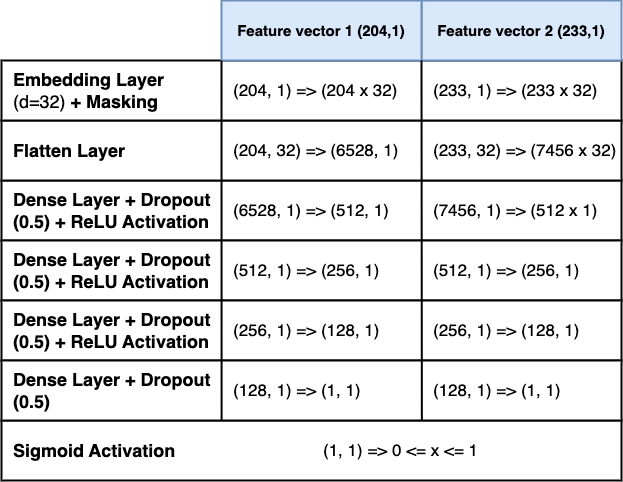
\includegraphics[width=0.7\textwidth]{images/DL.png}
  \end{center}
  \caption{This figure explains the deep learning model for both feature vectors. The different layers are shown on left column of the table. The input
  and output dimensions for each layer are shown in the other two columns.}
  \label{fig:modelStructure}
\end{figure}

By incorporating these additional features into our ML models, we aim to enhance the accuracy and effectiveness of
the tracking detection process, considering a broader range of contextual information associated with each request. 
Furthermore, every feature is known before a request is sent to the server and can be used to identify a tracking request
in real-time.

The deep neural network structure is almost identical to Castell-Uroz et al. \cite{castell2020url} and is illustrated in Fig-\ref{fig:modelStructure}.
The differences come from the different activation
function and the different input and output vector dimensions due to the different feature vectors. Like Castell-Uroz et al. we use an embedding layer to reduce the bias between the numerical values of the embedded URL string. This embedded 
representation then gets flattened into a one dimensional vector and put into the four dense layers. Each dense layer has a dropout rate of 50\% to reduce
overfitting and a ReLU\footnote{ReLU (Rectified Linear Unit) is a commonly used activation function in neural networks. It 
introduces non-linearity by outputting the input value if it is positive, and zero otherwise. ReLU is efficient and helps
networks learn complex patterns. It addresses the vanishing gradient problem but can suffer from the "dying ReLU" issue. Variants
like Leaky ReLU and Parametric ReLU exist to overcome this problem.} activation function. The last dense layer gets activated
by a Sigmoid\footnote{The sigmoid activation function is commonly used in neural networks for binary classification tasks. It maps input values to a range between 0 and 1, facilitating gradient-based optimization. However, it may encounter issues such as the vanishing gradient problem and asymmetry around zero. Despite these limitations, the sigmoid function remains a key component in neural network architectures.} function to generate an output
between zero and one.

By using the neural network structure of Castell-Uroz et al. we expect to achieve similar or better accuracy results with 
the newly crafted feature vector designs. However, it could be possible that the network architecture is not optimal
for the desired output and does not fit to the different feature vectors. There is a chance that a better architecture could 
lead to a better accuracy result and therefore would better fit the real-time application of the model. But ML architecture is beyond
the scope of this thesis and is an interesting topic for future work.

\subsection{Training-Data}

Selecting the appropriate training-data is a crucial step in the training of neural networks. The quality and representativeness 
of the training data directly impacts the performance and generalization ability of the network.

The utilization of the model in a real-time web environment necessitates the careful selection of the training dataset.
In our study, we sought to procure a dataset that aligns with the dynamics and characteristics of real-time web browsing.
To achieve this, we turned to a comprehensive web crawl conducted by Raschke \cite{raschke_philip_2022_7123945}, which involved the exploration and collection
of data from the Tranco \cite{pochat2018tranco} top 10K websites using the Chrome browser.

The choice of using a Chrome crawl dataset by Raschke holds several advantages for our model's training. Firstly, it is performed 
using the \emph{t.ex extension} \cite{9972261}, which is a cross browser extension and therefore runs in the same environment as our
application. Secondly, Chrome is one of the most widely used web browsers globally, making it a representative platform for
capturing the diverse range of web activities and behaviors.

Furthermore, the Chrome browser by default does not have any tracking protection associated. This leads to more tracking requests being executed
during the crawl which gives great potential for training a neural network. The dataset comes with 901,012 HTTP requests and responses all in JSON
format and a label to identify tracking requests from non tracking requests. Moreover, the dataset has been successfully used by Raschke et al. \cite{raschke2023}
to train a different tracker detection classifier.

For these reasons we decided to use this dataset \cite{raschke_philip_2022_7123945} to train our models and further on use these models
in the real-time application.

\subsection{Real-time Application}

For our real-time application, we focused on creating a cross browser extension. This comes close to current solutions in this area 
and provides a familiar entry point for users. 

\begin{figure}[ht!]
  \begin{center}
    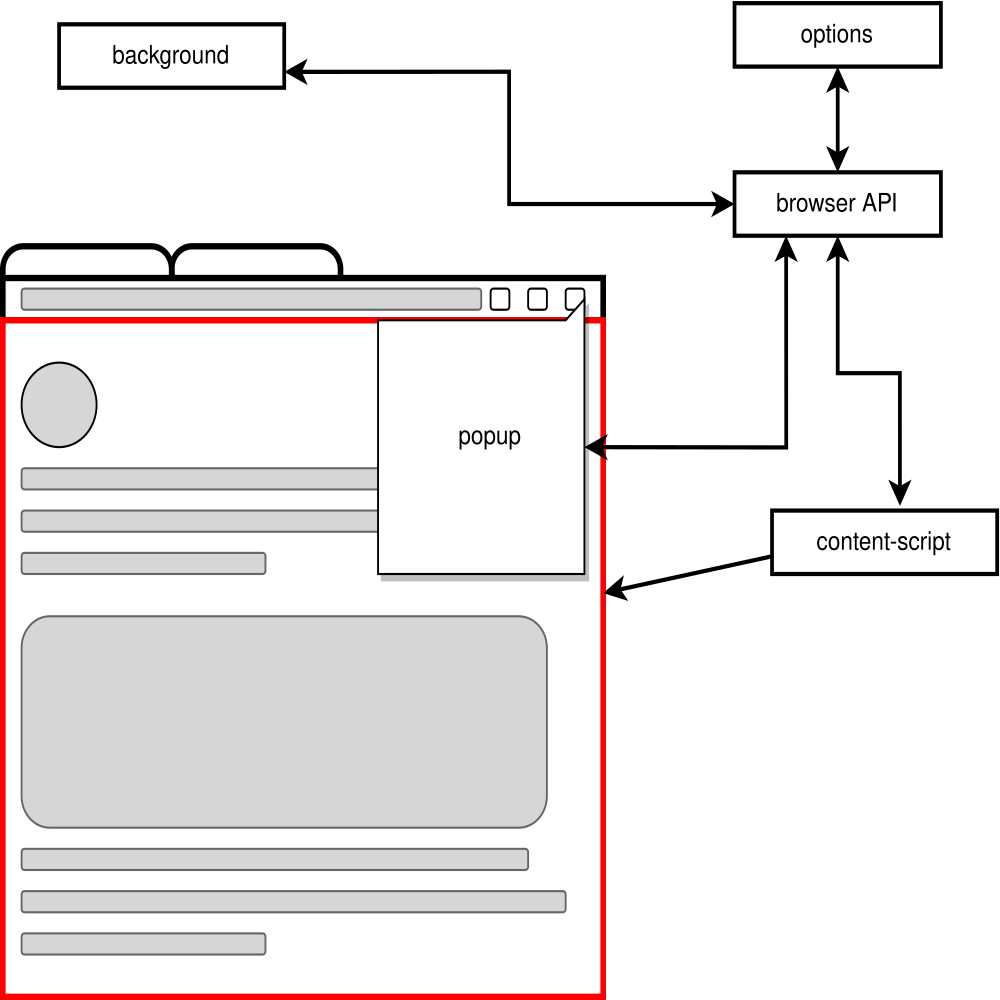
\includegraphics[width=0.75\textwidth]{images/ExtensionOverview.png}
  \end{center}
  \caption{This figure unveils the structure of a web extension and its most important components. There are user interface components which 
  can be used to communicate with the user of the extension such as the popup or the options page. Additionally, there is the content-script
which can be injected into each HTML page visited by the browser and the background page which can be used to implement the business logic of the extension. All the parts of the 
extension can communicate over the API provided by the browser.}
  \label{fig:extOver}
\end{figure}

Browser extensions are event based programs which can be used to enhance the browsing
experience. Moreover, browsers provide an API which can be used by the extension programmer to interact with the browser with JavaScript.
This API can then be used to block HTTP requests before they get sent to the server.

As shown in Fig-\ref{fig:extOver} a web extension may consist of a \emph{background} page, a \emph{popup}, \emph{option} pages and
content-scripts. Once the background script is loaded it can attach to various browser events and react accordingly. The browser API
provides numerous events \cite{browserApi} including events that allow to read and intercept HTTP requests. Another tool is  
\emph{content-scripts} which get directly injected every web page opened in the browser and can modify its content using
JavaScript. A web extension has two methods communicating with the user through a dedicated user interface. Firstly, it is possible
to provide a popup page to display information or controls. Secondly, it is possible to host an option-page or static HTML serving. This can
be used to provide the user more detailed options or more screen space.

We want to utilize the advantages of using a web extension as a real-time tracking blocker. Therefore, we implement a background script
which attaches to the \emph{onBeforeRequest} event to gather information about the request such as the \emph{requestId} and the source URL 
which initiated the request. Moreover, we use the \emph{onBeforeSendHeaders} event to block a request. Besides, the event callback provides
information about the request headers. With this information we then construct a feature vector and pass it to our ML model and cancel the 
request depending on the models' confidence. 

To improve usability we implement a popup to show the user the amount of trackers detected on a certain website and show
each request with the according confidence. Moreover, the user is able to regulate the threshold on which a request is determined a 
tracking request, and it is possible to enable or disable the blocking of web requests. By default, the application blocks every request
which got a confidence higher or equal to 80\%.

The implementation of this application heavily relies on \emph{TensorFlow.js} \cite{tensorflowJs} which is a library to port ML models to
JavaScript. This way we can calculate the feature vector and pass it to the TensorFlow layers model. This is extremely
performant as TensorFlow.js uses WebAssembly to calculate the model. This is an important factor in the real-time ability of this application.
With this concept, we meet the real-time criterion and hope to provide a seamless user-experience.

\subsection{Infrastructure}

As the web industry grows with rapid pace, also web tracker change in structure and technique. This could lead to the model being 
outdated as the training data is from a specific point of time. Another infrastructural problem is the use of TPLs as the ground truth. As mentioned
before these lists are error-prone and often just hide certain elements from the DOM. For that reason it is important to gather better 
training data with better labels. For that reason we also implemented an infrastructure to keep the model up to date and to enable user to
provide training data with custom labels.
\begin{figure}
  \begin{center}
    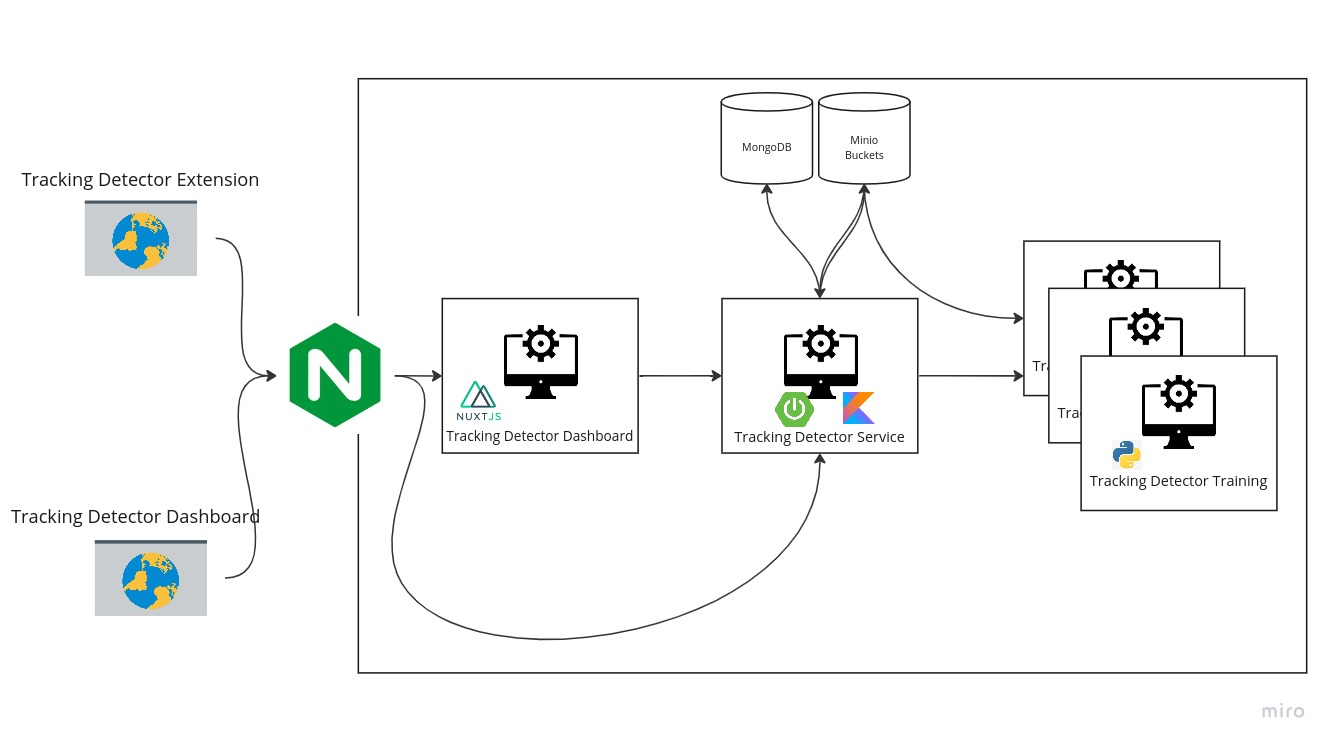
\includegraphics[width=1\textwidth]{images/TrackingDetectorInfra.jpg}
  \end{center}
  \caption{This figure depicts the architecture of the whole application. As for the client side we have the web extension and an admin panel to 
  monitor the learning rate. Every endpoint proxies through a NGINX gateway. The main service is in charge of storing new data into the training dataset and 
  to host the trained models. Furthermore, it is includes a job architecture which allows running different jobs based on a CRON pattern. For data storage there is 
  a bucket storage from \emph{MinIO} and a \emph{MongoDB} to hold the data the main service servers and modifies. Finally, there are multiple training services which are Python based
  these get triggered by the main service using \emph{XML-RPC}.
  }
  \label{fig:tdInfra}
\end{figure}

As shown in Fig-\ref{fig:tdInfra} a lot of thought went into the creation of a suitable backend infrastructure for the web extension. The goal of that
backend is to provide a simple way to train and deploy new ML models to the user of the web extension. The complete backend is divided into
three main services. The \emph{Tracking-Detector-Dashboard} is the administrator panel which allows the administrator to monitor learning rates and export 
training datasets. Through this panel it is also possible to trigger the job based architecture in the \emph{Tracking-Detector-Service}.

Another important aspect are two storage components within this
architecture. Firstly, the MongoDB\footnote{MongoDB is an open-source, NoSQL database system designed for storing and managing large volumes of flexible, JSON-like documents. It offers high scalability, fault tolerance, and rich querying capabilities, making it popular for modern applications like web and mobile apps, IoT devices, and big data analytics.}, which is NoSQL document database and is being utilized to store the raw browsing data of the clients and the ML model definitions which get 
trained. Furthermore, the statistics of each training run get stored in that database. The second storage component is a MinIO\footnote{MinIO is an open-source, high-performance object storage server compatible with Amazon S3 API. It is lightweight, easy to set up, and ideal for managing large unstructured data like images and videos. MinIO supports erasure coding and Bitrot protection for data durability and can be deployed on-premises or in the cloud. Its compatibility with S3 tools makes integration seamless, making it a popular choice for scalable and cost-effective storage solutions.} bucket storage service. This service 
is a scalable solution for storing all kinds of files.
This storage is utilized to export the raw training-data into easy to process CSV files which can be used to train the models. Moreover, the trained model
binaries get stored in that storage service.

The centerpiece of this backend is the \emph{Tracking-Detector-Service}. This service is in charge of processing new data points 
submitted by the users of the web extension and to gather them into a dataset which gets exported to the MinIO file storage. It also stores 
the original representation of the data points into a MongoDB such that any dataset representation can be created. Finally, this service
is in charge of serving the trained models to the clients, it does that by acting as an intermediate between the client and the MinIO service.
This service is implemented in Kotlin\footnote{Kotlin is a modern, statically-typed programming language designed by JetBrains. It is fully interoperable with Java, allowing seamless integration with existing codebases and libraries. Kotlin offers concise syntax, improved null safety, and enhanced type inference, making code more readable and safer. It is widely used for Android app development, server-side applications, web development, and more, with features like extension functions and coroutines for asynchronous programming, boosting productivity and expressiveness.} and uses the Spring Boot\footnote{Spring Boot is an open-source, Java-based framework for building production-ready Spring applications with streamlined configuration and faster development. It supports web applications, microservices, and RESTful APIs, facilitating easy deployment across environments and platforms, making it a popular choice for scalable Java applications.} framework to create a multithreaded server environment.
This framework has been chosen because of its testability and performance. Moreover, Spring Boot is industry standard for most backend systems and
provides solutions for almost any problem regarding server-side development.

The training of the models is done on one of the multiple \emph{Tracking-Detector-Training} services. These services are
lightweight XML-RPC\footnote{XML-RPC is a lightweight, remote procedure call (RPC) protocol that utilizes XML to encode data and communicate between software systems over networks. It enables easy integration between different platforms and programming languages, making it widely adopted in various applications. XML-RPC allows for simple and direct interactions, making it suitable for basic communication needs in distributed systems and web services.} server implemented in Python. The training gets started by an XML-RPC call to one of the services. After that, the service
grabs the training data from the MinIO storage bucket and compiles the ML model from the information provided by the XML-RPC call. It then starts
training the model and returns the model metrics to the \emph{Tracking-Detector-Service}.

As for the usability, we decided to wrap every component into a docker container and host the whole infrastructure in a \emph{docker-compose}
file which makes it easy to set up. This architecture can be used for all kind of ML based applications as the jobs are simple to extend 
and the creation of new models can be done via the admin panel. With this backend solution we hope to create an application that continuously creates
better models and serves them to the clients. We hope to simplify the process of gathering training data and to improve
ground truth in the web tracking field.

\subsection{Limitations}

However, there are limitations to this approach. The selected features may not be optimal for the problem and should be evaluated.
This could be done by generating variations of feature vectors using all the available features before a request is sent to the server.
After that, a grid search could be implemented to validate which feature vector fits the problem best. 

The same problem applies to the model. The neural network structure may not be optimal for the given use case and could also
be optimized with a grid search. This might lead to performance gains. Another more generic dataset could be used to create a better generalized
model which could improve performance in the real-time application causing less site breakages.

\section{Methodology}

In this section, we outline the methodology we employ to evaluate our models and real-time application for web tracker detection.
The methodology encompasses data collection, model training, evaluation metrics, and real-time application evaluation. By following
rigorous scientific methods, we aim to ensure the reliability, accuracy, and practicality of our models and application.

\subsection{Data Collection}
To gather the necessary data for evaluating our models and real-time application, we utilize a combination of approaches.
This involves conducting web crawls using browsers such as Chrome and Brave. Through these web crawls,
we collect a diverse set of web pages representing various domains. These crawls are being performed with Chrome without extensions,
Chrome with the first model, Chrome with the second model, Chrome with both models and a Brave which has built in advertisement and tracker blocking.
The crawler visits the Tranco \cite{pochat2018tranco} Top 1K websites and generate a browsing graph which includes the visited domains and the HTTP request
performed on each node.

\subsection{Model Training}
The training process involves preprocessing the dataset, including features extraction and
transformation into a suitable format for training the neural network models. We use the model architecture by Castell-Uroz et al. \cite{castell2020url}.
To ensure the generalizability of our models, we employ cross-validation techniques
to assess their performance on different subsets of the data.

\subsection{Evaluation Metrics}
To evaluate the performance of our models, we employ standard evaluation metrics commonly used in machine learning
classification tasks. These metrics include accuracy, precision, recall, F1-score, false positive rate, and false negative rate.
Accuracy measures the overall correctness of our models in identifying web trackers. Precision, recall, and F1-score provide
insights into the model's ability to accurately classify web trackers and non-trackers. The false positive rate and false negative
rate help assess the model's performance in minimizing false positives and false negatives, which directly impact user
experience and privacy.

\subsection{Real-time Application Evaluation}
In order to evaluate the performance of our real-time web tracker detection application, we examine the gathered data 
and look at the browsing graphs to determine the difference in the browsing experience.
Additionally, we measure the impact of the web extension on browsing performance, such as page load times and
resource consumption, to ensure minimal disruption to the user's browsing experience.






\chapter{Implementation}

\chapter{Evaluation}

\chapter{Conclusion}
\label{cha:conclusion}



%--------------------------------------------------------------
% TABLES, FIGURES, BIBLOGRAPHY AND APPENDICES
%--------------------------------------------------------------
\backmatter

% Lists of tables and figures


% Bibliography
\setwidesite{}						% Set page to be wider for bibliography
\markboth{Bibliography}{bibliography}
\label{cha:bibliography}
\bibliographystyle{IEEEtran}
\bibliography{bibliography.bib}
\chapter*{\LARGE Selbstständigkeitserklärung}
\begin{onehalfspace}
Hiermit erkläre ich, dass ich die von mir an der Provadis School of International Management and Technology AG eingereichte Seminararbeit zum Thema:
\begin{center}
\textbf{DevOps und CI / CD - Ein Einblick in DevOps und dessen Anwendung bei unterschiedlichen Unternehmen}
\end{center}
vollkommen selbständig verfasst und keine anderen als die angegebenen Quellen und Hilfsmittel benutzt habe.
Stellen, die wörtlich oder sinngemäß aus veröffentlichten oder noch nicht veröffentlichten Quellen entnommen sind, sind als solche kenntlich gemacht.
Die Abbildungen in dieser Arbeit sind von mir selbst erstellt oder mit einem entsprechenden Quellennachweis versehen.
Diese Arbeit ist in gleicher oder ähnlicher Form noch bei keiner anderen Hochschule/Universität eingereicht worden.

\vspace{30 mm}
\begin{flushright}

\rule{90mm}{1pt}

Frankfurt, \today \hspace{15 mm} Henry Schwerdtner
\end{flushright}

\end{onehalfspace}

% Use following to separate online (websites) and offline (books, papers) sources
%\printbibliography[heading=offline,filter=offline]
%\printbibliography[heading=online,filter=online]

%\begin{appendices}
%	\chapter{Appendix 1}
\section{Chrome Crawl}
\begin{figure}[ht!]
\begin{center}
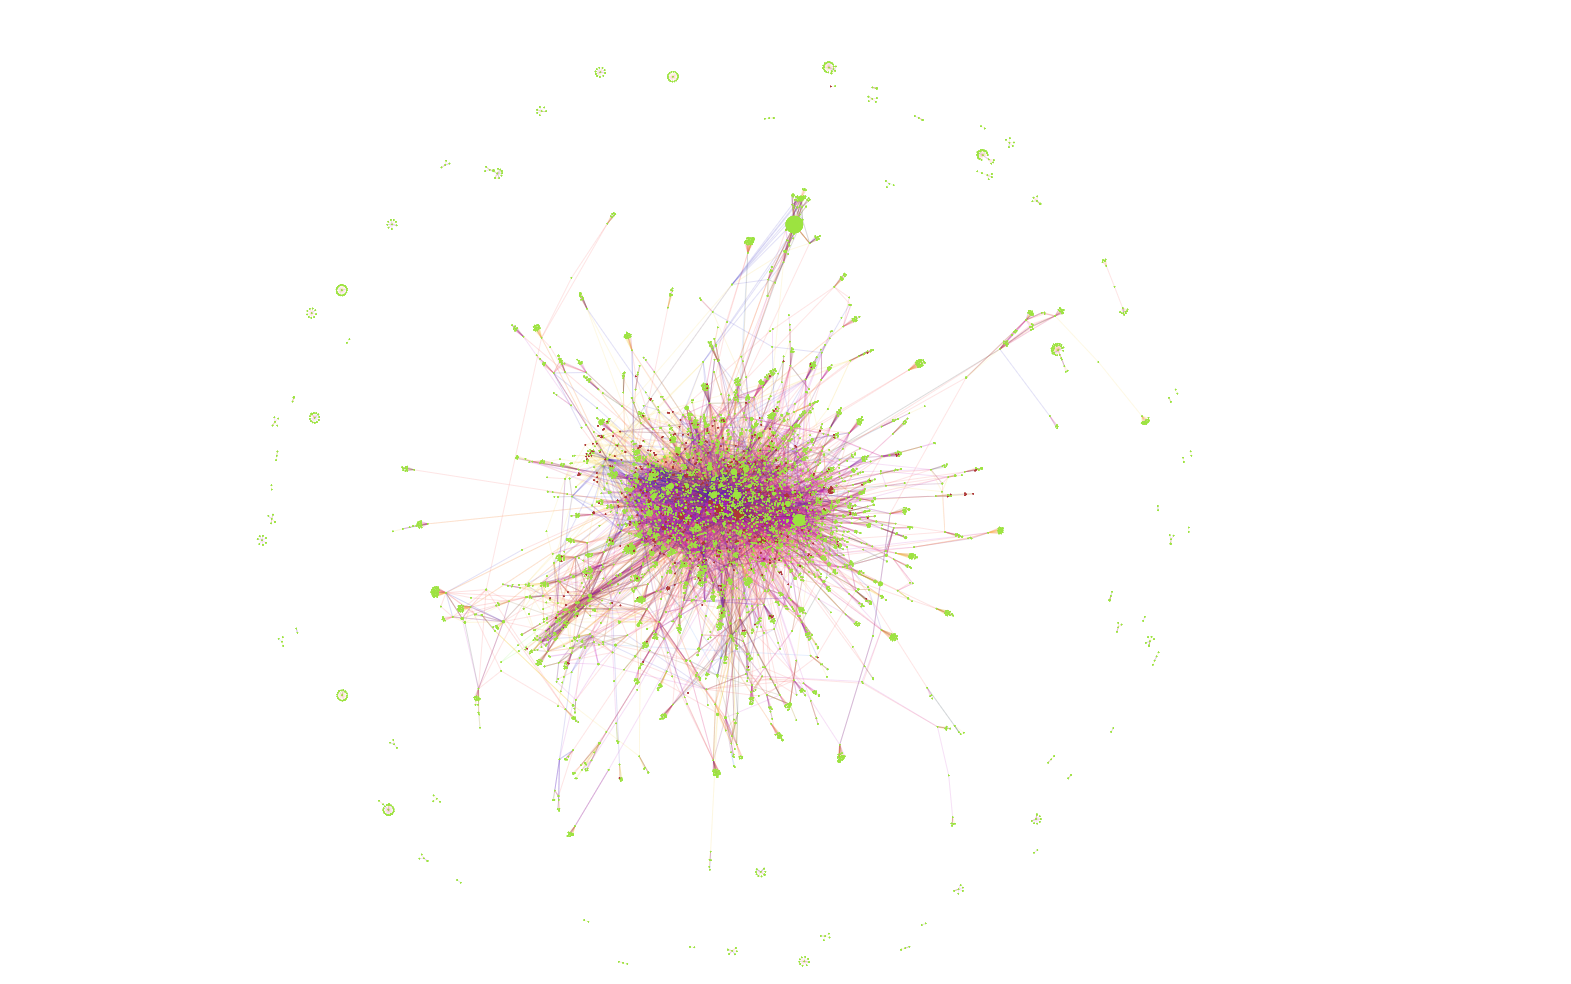
\includegraphics[width=0.75\textwidth]{images/chrome.png}
\end{center}
\caption{In this figure the browsing graph of the Tranco Top 1K websites, crawled on the Chrome browser, is visualized. }
\end{figure}
The Chrome crawl has been performed on the Tranco Top 1K websites. A fresh installation of the Chrome browser has been used to perform
the crawl. As for the statisitics, the Chrome browser visited \emph{5.546} unique domains and performed \emph{62.207} web request to 
visualize the one thousand different web pages. Of the requests \emph{1.518} were classified as tracking requests by the DuckDuckGo 
TPL and \emph{745} were classified by the EasyPrivacy TPL.

	% \chapter{Appendix 2}
\section{Brave Crawl}
\begin{figure}[ht!]
\begin{center}
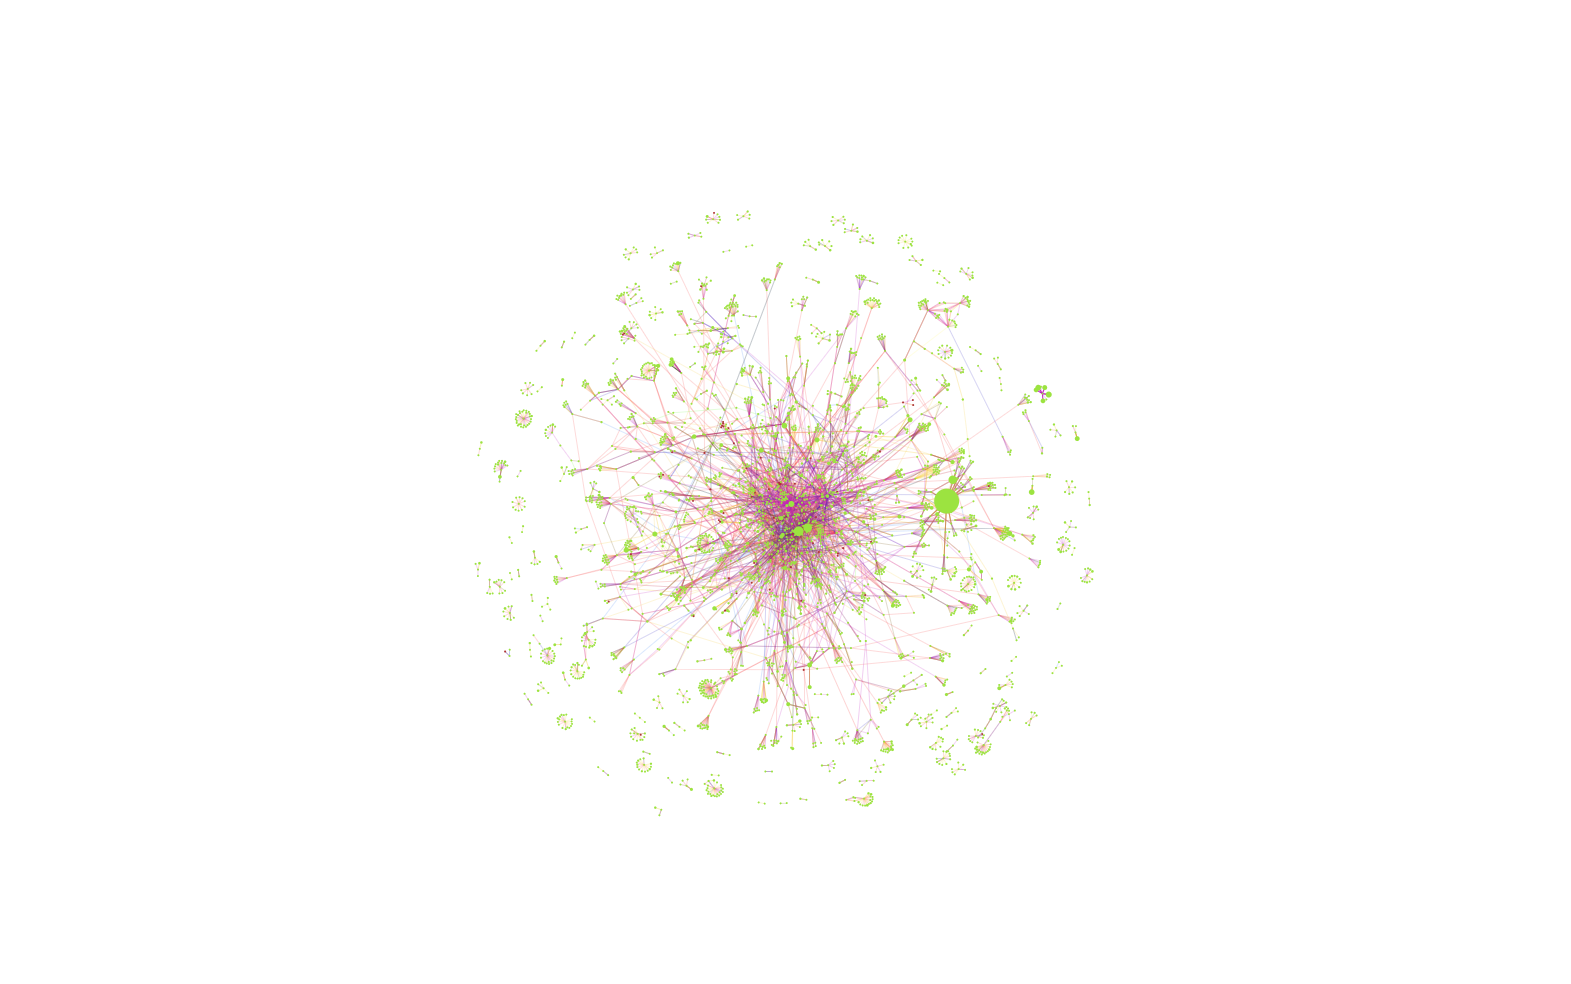
\includegraphics[width=0.75\textwidth]{images/brave.png}
\end{center}
\caption{In this figure the browsing graph of the Tranco Top 1K websites, crawled on the Brave browser, is visualized. }
\end{figure}
The Brave crawl has been performed on the Tranco Top 1K websites. A fresh installation of the Brave browser has been used to perform
the crawl. As for the statistics, the Brave browser visited \emph{3.678} unique domains and performed \emph{43.294} web request to 
visualize the one thousand different web pages. Of the requests \emph{588} were classified as tracking requests by the DuckDuckGo 
TPL and \emph{82} were classified by the EasyPrivacy TPL.

	% 
\chapter{Appendix 3}
\section{Chrome Model 1 Crawl}
\begin{figure}[ht!]
\begin{center}
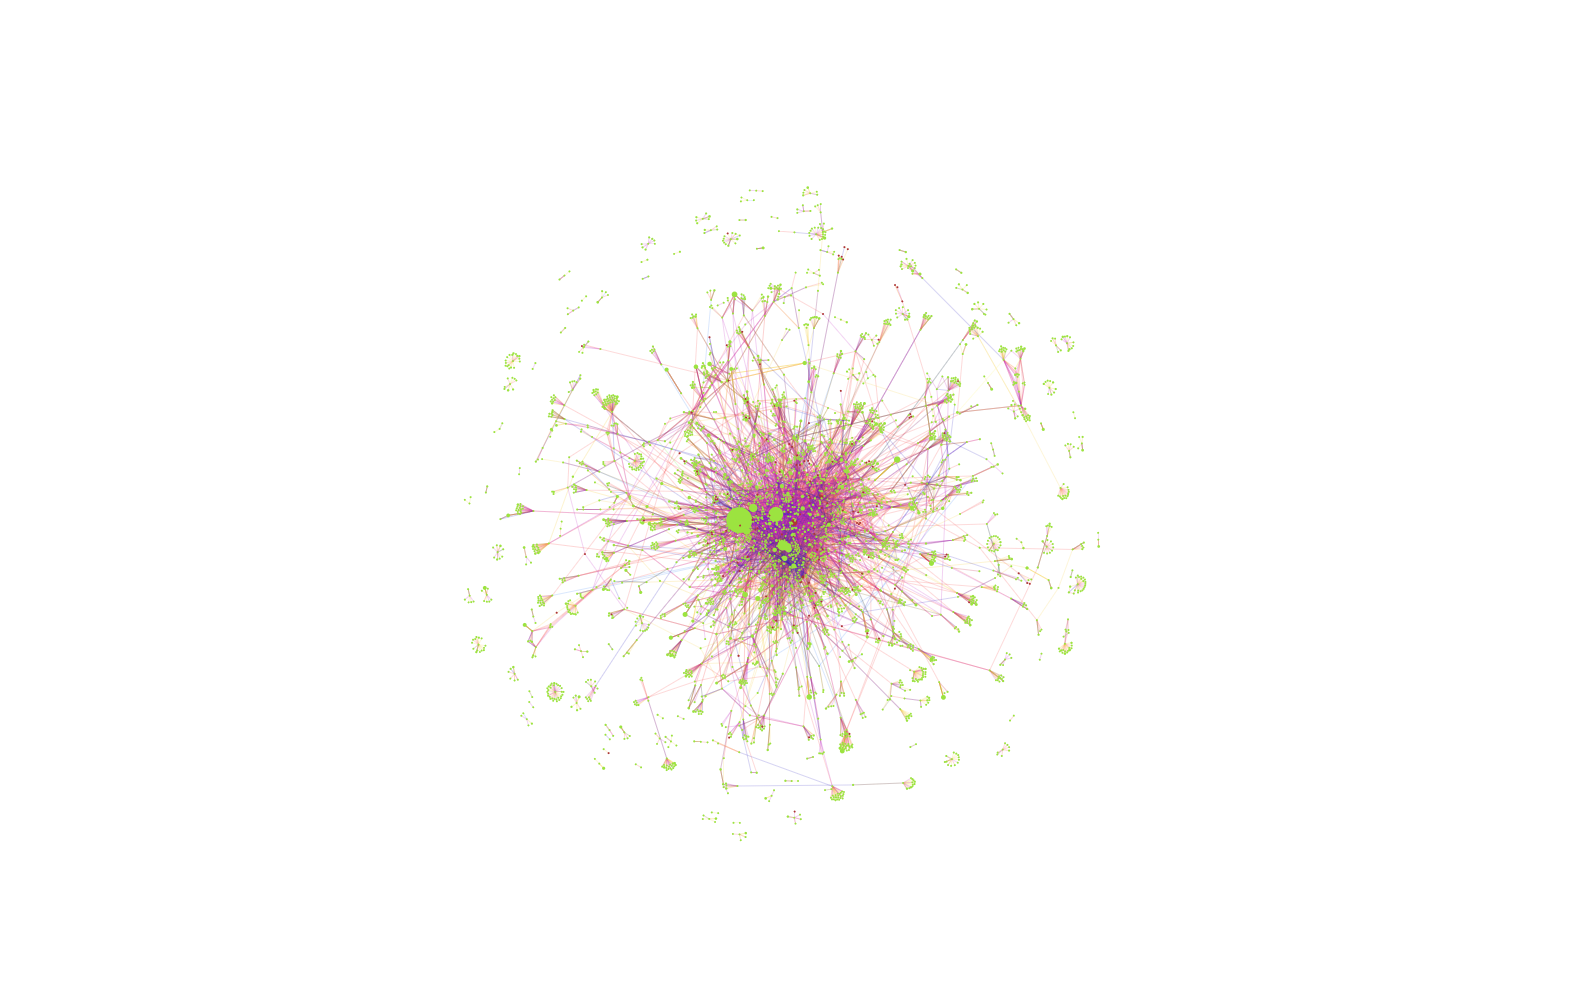
\includegraphics[width=0.75\textwidth]{images/original.png}
\end{center}
\caption{In this figure the browsing graph of the Tranco Top 1K websites, crawled on the Chrome browser with Model 1 active, is visualized. }
\end{figure}
The Brave crawl has been performed on the Tranco Top 1K websites. A fresh installation of the Chrome browser with Model 1 running in an extension has been used to perform
the crawl. As for the statistics, the Chrome browser with Model 1 active visited \emph{4.151} unique domains and performed \emph{47.255} web request to 
visualize the one thousand different web pages. Of the requests \emph{862} were classified as tracking requests by the DuckDuckGo 
TPL and \emph{213} were classified by the EasyPrivacy TPL.

%\end{appendices}

\end{document}
